\documentclass[12pt,a4paper]{article}
\usepackage[utf8]{inputenc}
\usepackage[T1]{fontenc}
\usepackage[magyar]{babel}
\usepackage{graphicx}
\usepackage{geometry}
\geometry{a4paper, margin=35mm, headheight=15mm}
\usepackage{fancyhdr}
\usepackage[hidelinks]{hyperref}
\usepackage[numbers]{natbib}
\usepackage{subcaption}

\pagestyle{fancy}
\fancyhf{}
\fancyhead[L]{\footnotesize\sc Vesetranszplantációs cserekörök egészértékű programozással}
\fancyhead[R]{\thepage}
\renewcommand{\headrulewidth}{0.4pt}
\renewcommand{\footrulewidth}{0pt}

\begin{document}

%% --------------------------------------------------------
%% Előlap
%% --------------------------------------------------------
\begin{titlepage}
\thispagestyle{empty}
\begin{center}


\includegraphics[height=18mm]{bme_logo_kicsi}

\vspace{2cm}

{\large\sc BSc Önálló Laboratórium Beszámoló}

\vspace{1.5cm}

{\LARGE\bf
Orvosi kritériumoknak megfelelő vesetranszplantációs cserekörök meghatározása egészértékű programozással
}

\vspace{1.5cm}

{\large Szigeti Tibor}

\vspace{1cm}

{\large Tanszéki konzulens: Nemkin Viktória}\\[0.3cm]
% {\large Külső konzulens: Biró Péter}

\vfill

{\sc Budapesti Műszaki és Gazdaságtudományi Egyetem\\
Villamosmérnöki és Informatikai Kar\\
Számítástudományi és Információelméleti Tanszék}

\vspace{0.8cm}

{\large Budapest, \the\year}

\end{center}
\end{titlepage}

%% --------------------------------------------------------
%% Tartalomjegyzék
%% --------------------------------------------------------
\tableofcontents
\newpage

%% --------------------------------------------------------
%% Tartalom
%% --------------------------------------------------------

\section{Bevezetés}
A laboratórium témája a vesetranszplantációs cserekörök meghatározására próbál megoldást adni. Ötletének forrása a páneurópai vesecsere program.

\subsection{Szakkifejezések}
\begin{itemize}
	\item Recipient-donor pair (RDP) - recipiens-donor pár
	
	A modellező gráfban is megjelenített ábrán a csúcspontokat alapvetően két személy alkotja. Egy donor és egy recipiens pár.

	\item Non-directed donors (NDD) / altruistic donors - altruista donor vagy önzetlen donor
	
	Olyan élő donor, aki nem egy konkrét személynek (például rokonnak vagy barátnak), hanem az országos/nemzetközi várólistán szereplő bármely rászoruló számára ajánlja fel a szervét.
\end{itemize}

\subsection{Modellező gráf}
Két ember egy pont, ami egy donort és egy recipienst jelent. A súlyozott, irányított élek a köztük lévő potenciális csere erőssége.

\begin{tabular}{c c}
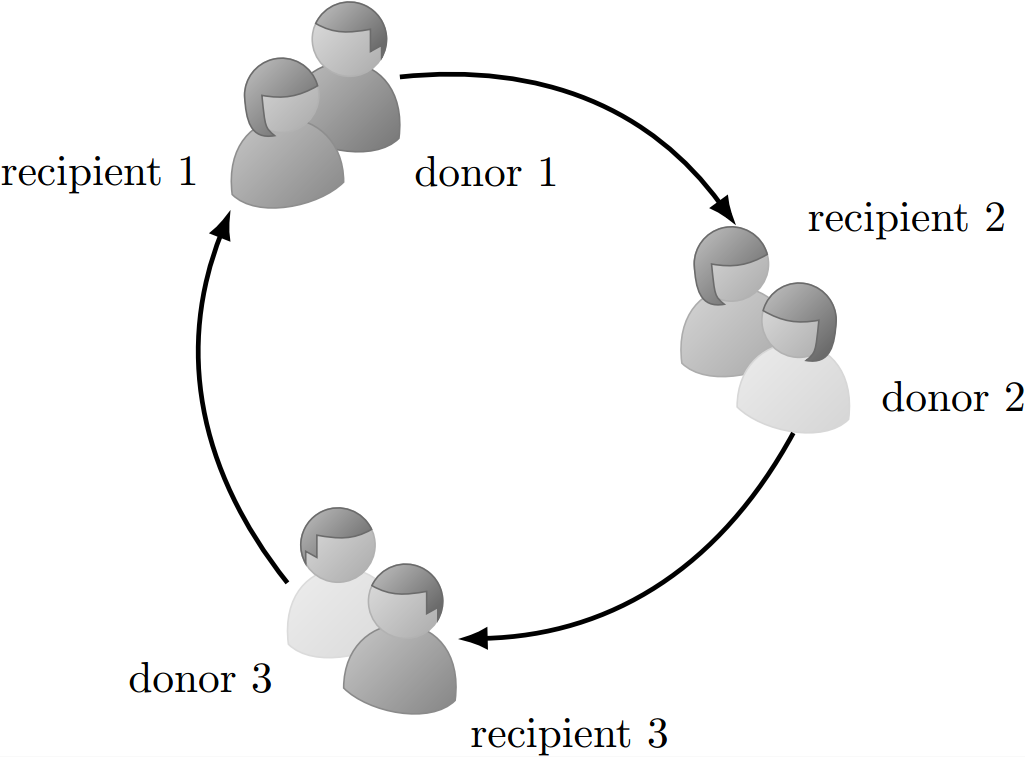
\includegraphics[width=62mm]{../docs/RDP-3pair-cycle} & 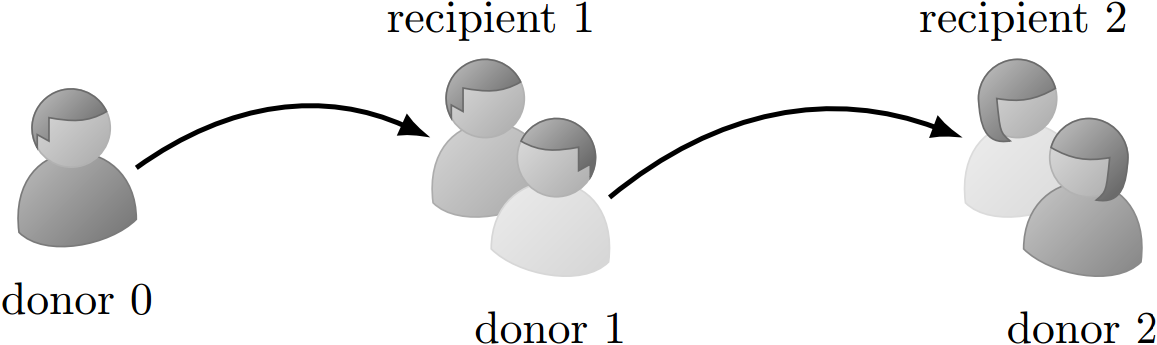
\includegraphics[width=62mm]{../docs/RDP-3pair-chain} \\
\end{tabular}

\subsection{Kezdeti kérdések}
Ahhoz, hogy a projekt használhatósága és a valóságot minél jobban modellező szemlélete megmaradjon az alábbi kérdéseket, majd válaszokat gyűjtöttem össze. Ezek segítenek a modell kialakítása során megtalálni a szükséges paramétereket és értékkészletüket.

\emph{Összefoglalás}

\section{Felhasznált adathalmaz}

A kezdeti kérdések alapján körvonalazódott modellezéshez a \href{https://researchdata.gla.ac.uk/1878/}{University of Glasgow vesecsere programok optimalizálásához szintetikusan előállított adathalmazát} használom fel, valamint bővítem ki.

\subsection{Adathalmaz jellemzése}

Tartalmaz egyes szintetikusan generált eseteket és felhasználási módja közé tartozik tesztelni és összehasonlítani különféle vesecsere program optimalizáló technikákat.

180 darab különböző vesecsere probléma esetet tartalmaz JSON formátumban. A JSON fájlok nevei egyben megadják az adott eset paramétereit is.
A nevek eleje egységesen:
uk\_2019\_splitpra\_bandxmatch\_pra0\_pdd,
majd egy alsóvonás jellel elválasztva követi az
<alt>\_<size>-<iteration>.json szöveg.
A relációs jelek közé írt értékek jelentése:
\begin{itemize}
	\item alt - altruista donorok aránya
	
	Értékkészlet: 0.05, 0.10, 0.20

	\item size - recipiensek száma
	
	Értékkészlet: 50, 100, 200, 500, 750, 1000

	\item iteration - különböző véletlenszerű esetek
	
	Értékkészlet: 0-9
\end{itemize}

\subsection{Jelenlegi adatmezők}

Minden JSON-fájl két fő részből áll. A donor-oldal (data) tartalmazza a dage mezőt (donor kora), a bloodtype mezőt (vércsoport: A, B, O vagy AB), az altruistic jelzőt (altruista donor-e), a sources mezőt (a hozzákapcsolt recipiens azonosítója, altruistáknál hiányzik), valamint a matches tömböt, amely az éleket írja le: minden él egy recipiens azonosítóból és egy score értékből áll. Ez utóbbi egy 0--100 közötti, előre aggregált kompatibilitási pontszám, valószínűleg UKLKSS-alapú HLA-mismatch érték.

A recipiens-oldal (recipients) tartalmazza a cPRA mezőt (kalkulált PRA-érték, 0 és 1 között), a bloodtype mezőt, valamint a hasBloodCompatibleDonor jelzőt, amely azt mutatja, van-e vércsoportilag kompatibilis donora az adott recipiensnek.

A jelenlegi solver kizárólag a gráfstruktúrát és az élsúlyokat (score) használja. A cPRA, dage, bloodtype és hasBloodCompatibleDonor mezők a jelenlegi modellben figyelmen kívül maradnak.

\subsection{Hiányzó mezők és lehetséges kiegészítések}

A recipiens kora (rage) hiányzik az adatokból, holott a donor--recipiens korkülönbség fontos minőségi kritérium, és a donor kora (dage) már elérhető. Szintetikus generálással pótolható UK KEP eloszlás alapján.

A várakozási idő (waiting\_time, napokban) a README szerint szerepelnie kellene, de a tényleges JSON-fájlokból hiányzik. Ez a Light-Equity optimalizálási policy egyik alapja lenne. UK historikus eloszlásból generálható.

A highly\_sensitised logikai jelző szintén ígérve van a README-ben, de nincs jelen. Triviálisan levezethető: cPRA értéke meghaladja-e a 0.85 küszöböt.

Az ország-azonosító (country) nélkülözhetetlen a páneurópai Egyéni Racionalitás elemzéséhez és az együttműködési politikák kiértékeléséhez. Szintetikusan hozzárendelhető, például 5 ország arányos elosztásával.

A távolság (distance\_km) él-szintű mező jelenleg nincs jelen, holott az EURO-KEP főváros-távolságot tervez közelítőként használni. Számítható, ha az ország-azonosító rendelkezésre áll.

HLA allél adatok (A, B, C, DR, DQ lókuszok) nem szerepelnek az adathalmazban, csak az aggregált score érték. Emiatt az Eurotransplant és a HLA Working Group pontszámok nem reprodukálhatók; a score valószínűleg UKLKSS-alapú.

A lemondási valószínűség (cancellation\_prob) él-szintű értékként nem szerepel. Lemondási politikák modellezéséhez szükséges lenne, és a cPRA értékéből élenkénti függvénnyel közelíthető.

A kompatibilis pár jelző (is\_compatible\_pair) nincs külön tárolva. A kompatibilis pár-politika (KEP-be lépési döntés minőségi feltétellel) szempontjából szükséges; a hasBloodCompatibleDonor mezőből részben következtethető.

Az LKDPI összetevői (magasság, súly, vérnyomás, eGFR, dohányzás) nem elérhetők, csak a donor kora (dage) áll rendelkezésre. A teljes LKDPI-index így nem számítható.

A centrum-azonosító (center\_id) sem szerepel az adatokban, holott a különböző transzplantációs centrumok eltérő kapacitáskorlátokkal rendelkezhetnek. Szintetikusan hozzárendelhető.

\subsection{Amit a solver már most felhasználhatna}

A cPRA értéke alapján az erősen érzékenyített recipiensek (cPRA nagyobb mint 0.85) preferálhatók lennének az objektívfüggvényben, például egy bónusztaggal súlyozva az élsúlyt.

Ha a recipiens kora (rage) is megvolna, a donor--recipiens korkülönbség beépíthető lenne élsúlyként.

A hasBloodCompatibleDonor jelző alapján a kompatibilis párok azonosíthatók, és más belépési feltételekkel kezelhetők: csak akkor lépnek be a KEP-be, ha a csere minőségi javulást hoz, és legfeljebb 1--3 futtatáson maradnak.

A cPRA-ból per-él lemondási valószínűség számítható. Ekkor az objektív nem a nyers score-t, hanem a várható értéket maximalizálja, azaz a score és az 1 mínusz a lemondási valószínűség szorzatát.

\begin{figure}[htbp]
  \centering
  \begin{subfigure}[b]{0.42\textwidth}
    \centering
    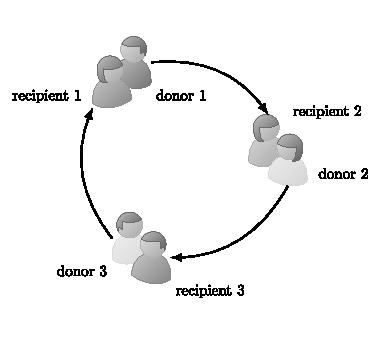
\includegraphics[width=\linewidth]{Figures/cycle}
    \caption{Example of a cycle~\cite[Figure~1]{barkel2026}.}
  \end{subfigure}
  \hfill
  \begin{subfigure}[b]{0.54\textwidth}
    \centering
    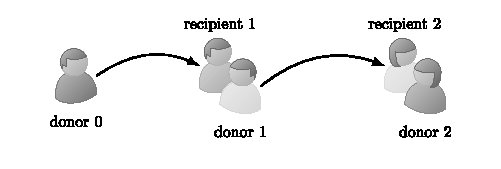
\includegraphics[width=\linewidth]{Figures/chain}
    \caption{Example of a chain~\cite[Figure~2]{barkel2026}.}
  \end{subfigure}
\end{figure}

\bibliographystyle{abbrvnat}
\bibliography{X6E3NN}

\end{document}
